\documentclass[12pt,letterpaper]{article}

\usepackage[spanish, es-nodecimaldot]{babel}
\usepackage[utf8]{inputenc}
\usepackage[T1]{fontenc}
\usepackage{lmodern}
\usepackage{amssymb, amsmath}
\usepackage{geometry}
\geometry{margin=1in}
\usepackage{setspace}
\onehalfspacing
\usepackage{float}
\setlength{\parskip}{0.25em}
\usepackage{graphicx}
\usepackage{xcolor}
\usepackage{tabularx}
\usepackage{booktabs}
\renewcommand{\arraystretch}{1.25}
\setlength{\tabcolsep}{8pt}
\newcolumntype{Y}{>{\raggedright\arraybackslash}X}
\usepackage{xurl}
\usepackage{hyperref}
\usepackage{enumitem}
\usepackage{titlesec}
\usepackage{verbatim}
\titleformat{\section}{\large\bfseries}{\thesection.}{0.5em}{}
\titleformat{\subsection}{\normalsize\bfseries}{\thesubsection}{0.5em}{}
\titleformat{\subsubsection}{\normalsize\itshape}{\thesubsubsection}{0.5em}{}
\usepackage{fancyhdr}
\pagestyle{fancy}
\fancyhf{}

\newcommand{\universidad}{Pontificia Universidad Javeriana}
\newcommand{\facultad}{Facultad de Ingeniería}
\newcommand{\carrera}{Ingeniería de Sistemas}
\newcommand{\curso}{Visualización de Datos}
\newcommand{\proyecto}{Análisis y visualización de delitos en Bogotá}
\newcommand{\subtitulo}{Segunda Entrega -- Proyecto Final}
\newcommand{\profesor}{Laura Gomez}
\newcommand{\autores}{Luis Gutiérrez \\ Emilio Vargas \\ Santiago Suarez}
\newcommand{\fechaentrega}{Bogotá, Abril de 2026}
\newcommand{\abreviaturaCurso}{Visualización de Datos}

\hypersetup{
  colorlinks=true,
  linkcolor=black,
  urlcolor=blue,
  citecolor=black,
  pdfauthor={\autores},
  pdftitle={\proyecto}
}

\fancyhead[L]{\small \abreviaturaCurso}
\fancyhead[R]{\small \universidad}
\fancyfoot[C]{\thepage}

\sloppy

\begin{document}

\begin{titlepage}
  \centering
  \vspace*{0.5cm}
  \includegraphics[width=5cm]{logo_javeriana.png}\par
  \vspace{0.5cm}
  {\Large \universidad \par}
  {\large \facultad \par}
  {\large \carrera \par}
  \vspace{2.0cm}
  {\Large \textbf{\proyecto}\par}
  \vspace{0.5cm}
  {\large \textbf{\subtitulo}\par}
  \vspace{0.8cm}
  {\large \textbf{Asignatura:} \curso\par}
  \vspace{0.8cm}
  {\large \textbf{Autores:}\par}
  {\large \autores\par}
  \vspace{0.8cm}
  {\large \textbf{Profesor:} \profesor\par}
  \vfill
  {\large \fechaentrega\par}
\end{titlepage}

\setcounter{page}{1}
\tableofcontents
\newpage

%==============================================================================
\section{Ajustes derivados de la retroalimentación}
%==============================================================================

\textit{[Pendiente: describir los cambios incorporados a partir de los comentarios de la primera entrega (por ejemplo, precisión del alcance, fuentes de datos, redacción del modelo o preguntas generadoras).]}

%==============================================================================
\section{Introducción}
%==============================================================================

\textit{[Pendiente: propósito del documento, alcance del proyecto (Bogotá, hurtos, OLSC-Bogotá, UPZ), estructura del informe y puente narrativo hacia el contexto y el problema.]}

%==============================================================================
\section{Contexto}
%==============================================================================

\subsection{Sector de seguridad ciudadana}

El proyecto se desarrolla en el sector de seguridad ciudadana, enfocado en el análisis de delitos de alto impacto y hurto a personas en Bogotá. Este sector busca reducir la criminalidad y mejorar la calidad de vida mediante el uso de información y herramientas analíticas que permiten entender mejor el comportamiento del delito. Se trata de situaciones que impactan cómo las personas perciben la seguridad, y son situaciones que demandan acciones operativas permanentes tanto de monitoreo como de reacción. El propósito principal es identificar patrones en el espacio y el tiempo, comprender los aumentos repentinos y las variaciones en los tipos de delito, y convertir ese análisis en una asignación zonal prioritaria. Así, es posible tomar decisiones fundamentadas en información real sobre la manera en que se distribuyen los recursos y los programas gubernamentales orientados a garantizar la seguridad en Bogotá.

\subsection{Organización: OLSC-Bogotá}

Inicialmente se delimita el alcance del análisis en la visualización en las UPZ como unidad base. Los conjuntos de datos seleccionados permiten principalmente calcular tasas por cada 100 mil habitantes (cuando se dispone de población), densidad por kilómetro cuadrado, identificar tendencias, variaciones por día y hora, correlaciones entre los llamados de emergencia al 123 y los delitos, y comparar antes y después de intervenciones.

Con base en lo anterior, se define la organización en donde aplicar el proyecto: el Observatorio Local de Seguridad y Convivencia de Bogotá (OLSC-Bogotá), cuyo objetivo es ordenar, documentar y analizar fuentes de información ya existentes, articular sus clasificaciones y generar productos de inteligencia aplicada. Entre estos productos se incluyen informes ejecutivos mensuales, seguimiento a las modalidades delictivas en Bogotá, e identificación de señales de demanda ciudadana provenientes de la línea 123, con el fin de alimentar los comités locales de seguridad. La unidad de análisis prioritaria es la UPZ, lo cual se alinea con la estructura de planeación urbana del Distrito y los planes de acción zonales.

%==============================================================================
\section{Problema}
%==============================================================================

En la organización seleccionada, existe un flujo de trabajo compuesto de cuatro etapas:

\begin{enumerate}[label=\roman*.]
    \item Adición y estandarización de datos (incluyendo fechas, territorios, categorías y dominios)
    \item Modelado relacional y dimensional con adición de variables temporales y espaciales
    \item Análisis exploratorio para la evaluación de completitud, consistencia y patrones de los datos
    \item Difusión de resultados mediante paneles interactivos y boletines de alerta.
\end{enumerate}

Este proceso y los análisis que realizan tienen como usuarios destino a coordinadores y analistas de seguridad zonales, así como actores académicos o comunitarios que necesiten soluciones que sean medibles y comparables en el tiempo y en el espacio. Adicionalmente, la función que realiza el OLSC en colaboración con las entidades gubernamentales es la de recopilar sus datos y utilizarlos para liderar soluciones en la gestión de la seguridad y las emergencias.

Teniendo en cuenta todo lo mencionado, se detectan ciertas necesidades de la organización:

\begin{itemize}
    \item Integración de fuentes específicas y dispersas para relacionar los incidentes reportados y recopilados en bases de datos con lo que se registra como delito.
    \item Visualizaciones funcionales con múltiples filtros específicos tanto por UPZ, franjas horarias y mapas.
    \item Reportes formales para análisis por juntas de acción comunal y para el seguimiento de las intervenciones pertinentes.
\end{itemize}

\section{Objetivos del proyecto}

\subsection{Objetivo general}

Desarrollar un sistema de análisis y visualización de datos sobre hurtos a personas en Bogotá para apoyar la toma de decisiones estratégicas en el ámbito de seguridad en la ciudad.

\subsection{Objetivos específicos}

\begin{enumerate}
    \item Recopilar, limpiar y modelar conjuntos de datos provenientes de diversas fuentes (Datos Abiertos Bogotá, NUSE 123).
    \item Desarrollar indicadores clave para analizar patrones temporales, diferencias entre territorios y relaciones entre los delitos y las solicitudes de las personas.
    \item Crear dashboards interactivos que permitan visualizar la información con filtros ajustables y mapas a nivel de UPZ.
    \item Validar el sistema mediante la retroalimentación de usuarios por medio de encuestas para evaluar su utilidad en la gestión de seguridad local.
\end{enumerate}

\section{Objetivos de analítica y visualización}

\begin{enumerate}
    \item \textbf{Prioridad de zonas por UPZ:} Identificar la concentración de eventualidades para priorizar zonas, combinando conteos con las delimitaciones de las UPZ, y normalizando por habitantes.
    \item \textbf{Ritmos semanales y franjas horarias:} Analizar la distribución de incidentes por día de semana y por franjas horarias para optimizar turnos y patrullajes según la modalidad.
    \item \textbf{Tendencia temporal por tipo de delito:} Desarrollar series temporales (mensuales y anuales) por tipo de delito para entender evolución, estacionalidad y posibles puntos de cambio.
    \item \textbf{Evaluación de intervenciones:} Medir el efecto de intervenciones seleccionadas (reales o simuladas) sobre indicadores clave, comparando ventanas con fechas antes y después.
    \item \textbf{Línea 123 como alerta temprana:} Evaluar si la demanda de las personas al 123 anticipa el comportamiento de los delitos registrados en las zonas de la ciudad.
\end{enumerate}

%==============================================================================
\section{Preguntas generadoras}
%==============================================================================

\begin{enumerate}
    \item ¿En qué UPZ se concentran los eventos de inseguridad de manera crítica, y cuáles deberían priorizarse para la asignación de recursos gubernamentales?
    \item ¿Cuáles son los días de la semana y las franjas horarias donde se concentran los diferentes tipos de delito, y en qué momentos críticos conviene reforzar los recursos de vigilancia y patrullaje?
    \item ¿Cómo ha evolucionado la incidencia de cada tipo de delito en Bogotá, y cuáles han sido los cambios de tendencia que permiten evaluar el impacto de intervenciones futuras?
    \item ¿Las intervenciones de seguridad implementadas (reales o simuladas) han generado una reducción significativa en los indicadores clave como densidad delictiva, tasa por 100 mil habitantes o índice de franjas horarias críticas?
    \item ¿En qué categorías de delito y en qué UPZ la demanda ciudadana registrada a través de la línea 123 anticipa el comportamiento de los delitos formalmente denunciados?
\end{enumerate}

%==============================================================================
\section{Conjuntos de datos y preparación}
%==============================================================================

\subsection{Descripción de las fuentes}

El primer dataset utilizado corresponde a los registros de hurtos en Bogotá durante el año 2025. Este conjunto de datos contiene información detallada sobre los eventos de hurto, incluyendo variables como la fecha del hecho, el género de la víctima, el grupo etario, el tipo de arma o medio utilizado, el departamento, el municipio, el código DANE y la cantidad de casos reportados. Este dataset es fundamental para el proyecto, ya que permite analizar la dinámica de la criminalidad en la ciudad, identificar patrones temporales y segmentar los incidentes según características demográficas y contextuales.

Los conjuntos de datos utilizados están disponibles en las siguientes fuentes:
\begin{itemize}[noitemsep, topsep=0pt]
    \item Estadística delictiva (Policía Nacional de Colombia): \url{https://www.policia.gov.co/estadistica-delictiva}
    \item Delito de Alto Impacto (Datos Abiertos Bogotá): \url{https://datosabiertos.bogota.gov.co/dataset/delito-de-alto-impacto-bogota-d-c}
    \item Incidentes tramitados en el C4 -- NUSE (Datos Abiertos Bogotá): \url{https://datosabiertos.bogota.gov.co/dataset/incidentes/resource/30d65a8b-d0ed-4e95-977e-0d7cc2ea89ef}
\end{itemize}

El segundo dataset corresponde a las llamadas realizadas a la línea de emergencias 123 (C4). Este conjunto de datos incluye información sobre los incidentes reportados por la ciudadanía, tales como el tipo de evento, la fecha y hora de la llamada, la ubicación y en algunos casos una descripción del suceso. Este dataset aporta una perspectiva complementaria al análisis, ya que permite estudiar la percepción ciudadana de seguridad y contrastar con los registros oficiales de hurtos, facilitando la identificación de posibles diferencias entre los eventos reportados y los registrados.

El tercer dataset corresponde a la División Administrativa de Bogotá a nivel de Unidades de Planeamiento Zonal (UPZ). Este dataset contiene información geográfica, incluyendo la delimitación espacial de cada UPZ mediante geometrías, así como identificadores de cada zona. Su principal utilidad dentro del proyecto es permitir la georreferenciación de los datos, facilitando la construcción de mapas y el análisis espacial de los delitos, lo que resulta clave para identificar zonas con mayor incidencia de hurtos y apoyar la toma de decisiones territoriales.

\subsection{Preparación y limpieza de datos}

\textit{[Pendiente: documentar el proceso ETL. Sugerencia de contenido:]}
\begin{itemize}
    \item Ingesta y formatos de los archivos originales.
    \item Depuración: valores nulos, duplicados y registros atípicos.
    \item Estandarización: fechas, códigos DANE, nombres de UPZ y categorías.
    \item Georreferenciación y cruce espacial con el dataset de UPZ.
    \item Variables derivadas: tasas por 100\,000 habitantes, densidad, franjas horarias, agregaciones temporales.
    \item Control de calidad: completitud, consistencia y validaciones cruzadas entre fuentes.
    \item Herramientas utilizadas (por ejemplo, Python, R, Excel, Power Query).
\end{itemize}

\subsection{Integración de los conjuntos de datos}

La integración de estos datasets se realiza a partir de variables comunes como la ubicación geográfica (código DANE, municipio o UPZ) y la dimensión temporal (fecha de los eventos). Esta integración permite construir un modelo de datos unificado que facilita el análisis de todo este conjunto de datos que representa el fenómeno de seguridad, combinando información de hechos delictivos, percepción ciudadana y distribución espacial.

%==============================================================================
\section{Modelo lógico de datos final}
%==============================================================================

\subsection{Cambios respecto a la primera entrega}

\textit{[Pendiente: describir ajustes al modelo (nuevas entidades, atributos, relaciones o correcciones) derivados del trabajo de integración y limpieza.]}

\subsection{Descripción del modelo}

El modelo lógico de datos propuesto tiene como objetivo integrar información proveniente de diferentes fuentes para permitir el análisis del fenómeno de seguridad en Bogotá desde una perspectiva temporal, demográfica y geográfica. Para ello, se definieron cuatro entidades principales: \textbf{HECHOS-HURTO, LLAMADAS-123, UBICACION y UPZ,} las cuales se relacionan entre sí para estructurar la información de manera coherente y facilitar su análisis.

La entidad \textbf{HECHOS-HURTO} representa los registros oficiales de hurtos y constituye una de las tablas principales del modelo. En esta se almacenan variables clave como la fecha del hecho, el género de la víctima, el grupo etario, el tipo de arma utilizada y la cantidad de casos. Además, incluye el campo \textbf{codigo-dane}, que permite relacionar cada registro con su respectiva ubicación geográfica.

Por su parte, la entidad \textbf{LLAMADAS-123} contiene la información correspondiente a los reportes ciudadanos realizados a la línea de emergencias. Esta tabla incluye datos como la fecha del incidente, el tipo de evento reportado y su ubicación, también referenciada mediante el codigo-dane. Esta entidad complementa el análisis al aportar una visión desde la percepción ciudadana, permitiendo contrastar los datos oficiales con los reportes realizados por la comunidad.

La entidad \textbf{UBICACION} actúa como una tabla intermedia que centraliza la información geográfica, incluyendo el municipio, el departamento y la referencia a la UPZ correspondiente. Esta entidad es clave dentro del modelo, ya que permite unificar la información espacial de los distintos datasets y establecer relaciones entre ellos a través del codigo-dane.

Como último se usa la entidad \textbf{UPZ} que contiene la información geográfica detallada de las Unidades de Planeamiento Zonal, incluyendo su identificador, nombre y geometría. Esta tabla permite realizar análisis espaciales más específicos y facilita la construcción de visualizaciones geográficas, como mapas de calor o distribuciones por zonas.

En cuanto a las relaciones, tanto la entidad \textbf{HECHOS-HURTO} como \textbf{LLAMADAS-123} se conectan con \textbf{UBICACION} mediante una relación de muchos a uno, ya que múltiples registros pueden pertenecer a una misma ubicación. A la vez, \textbf{UBICACION} se relaciona con \textbf{UPZ} también en una relación de muchos a uno, permitiendo agrupar diferentes ubicaciones dentro de una misma zona geográfica.

\begin{figure}[H]
  \centering
  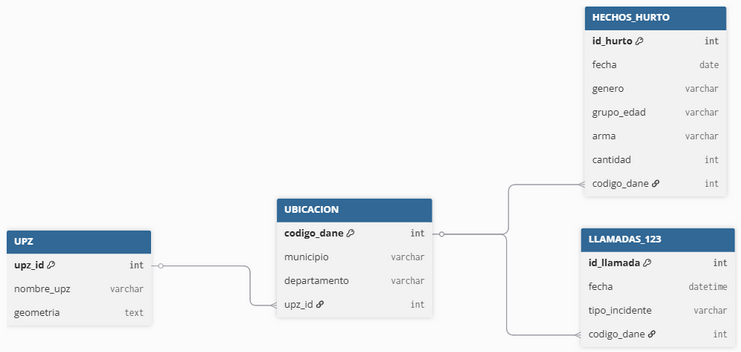
\includegraphics[width=16cm]{modelo-datos.png}
  \caption{Modelo lógico de datos del proyecto.}
  \label{fig:modelo-datos}
\end{figure}

%==============================================================================
\section{Registro de la visualización análoga en vivo}
%==============================================================================

\subsection{Diseño de la actividad}

\textit{[Pendiente: qué se observó o recolectó, dónde, cuándo y con qué protocolo.]}

\subsection{Evidencias}

\textit{[Pendiente: insertar fotografías, notas de campo y registros de la actividad.]}

\subsection{Resultados}

\textit{[Pendiente: hallazgos cuantitativos y cualitativos de la recolección en vivo.]}

\subsection{Reflexión metodológica}

\textit{[Pendiente: utilidad de la técnica, limitaciones (sesgo, muestra, horario, cobertura) y comparación con datos oficiales o del 123.]}

\subsection{Integración al análisis del proyecto}

\textit{[Pendiente: cómo los resultados de la visualización análoga alimentan preguntas generadoras u objetivos de analítica.]}

%==============================================================================
\section{Dashboard dinámico}
%==============================================================================

\textit{[Pendiente: herramienta utilizada, enlace de acceso y descripción general del tablero.]}

\subsection{Pantallas por objetivo de analítica}

\textit{[Pendiente: mínimo una pantalla por cada objetivo de analítica. Incluir capturas y breve interpretación.]}
\begin{itemize}
    \item \textbf{Objetivo 1 -- Prioridad de zonas por UPZ:} [nombre de pantalla / captura].
    \item \textbf{Objetivo 2 -- Ritmos semanales y franjas horarias:} [nombre de pantalla / captura].
    \item \textbf{Objetivo 3 -- Tendencia temporal por tipo de delito:} [nombre de pantalla / captura].
    \item \textbf{Objetivo 4 -- Evaluación de intervenciones:} [nombre de pantalla / captura].
    \item \textbf{Objetivo 5 -- Línea 123 como alerta temprana:} [nombre de pantalla / captura].
\end{itemize}

\subsection{Filtros dinámicos}

\textit{[Pendiente: documentar al menos cuatro filtros por categorías, por ejemplo UPZ, tipo de delito, periodo y franja horaria.]}

%==============================================================================
\section{Reporte ejecutivo}
%==============================================================================

\textit{[Pendiente: referenciar el PDF anexo del reporte ejecutivo. Resumir indicadores clave y estadísticas principales alineadas con los objetivos del proyecto.]}

%==============================================================================
\section{Conclusiones y recomendaciones}
%==============================================================================

\subsection{Conclusiones}

\textit{[Pendiente: conclusiones vinculadas a preguntas generadoras y objetivos de analítica.]}

\subsection{Recomendaciones}

\textit{[Pendiente: recomendaciones operativas para el OLSC-Bogotá y actores de seguridad local.]}

%==============================================================================
\section{Lecciones aprendidas}
%==============================================================================

\textit{[Pendiente: reflexión sobre el proceso técnico, el trabajo en equipo, limitaciones del estudio y trabajo futuro.]}

%==============================================================================
\section{Anexos}
%==============================================================================

\textit{[Pendiente: listar y entregar los archivos adjuntos requeridos por el enunciado.]}
\begin{itemize}
    \item Datasets procesados: \texttt{[ruta o nombre de archivo]}.
    \item Modelo de datos: \texttt{[diagrama, DDL o archivo del modelo]}.
    \item Dashboard / visualizador: \texttt{[archivo .pbix, .twbx, URL, etc.]}.
    \item Reporte ejecutivo en PDF: \texttt{[nombre del archivo]}.
    \item Evidencias de visualización análoga: \texttt{[carpeta o archivos]}.
\end{itemize}

\addcontentsline{toc}{section}{Referencias}
\begin{thebibliography}{99}
\raggedright

\bibitem{cisc2025} 
Cisc. (2025). \textit{Estadística delictiva | Policía Nacional de Colombia}. Policía Nacional De Colombia. \url{https://www.policia.gov.co/estadistica-delictiva}

\bibitem{datosbog_altoimpacto}
\textit{Delito de Alto Impacto. Bogotá D.C. - Datos Abiertos Bogotá}. (s.f.). \url{https://datosabiertos.bogota.gov.co/dataset/delito-de-alto-impacto-bogota-d-c}

\bibitem{datosbog_nuse}
\textit{Incidentes Tramitados en el C4 - Numero Único de Seguridad y Emergencia. NUSE. Bogotá D.C. - Datos Abiertos Bogotá}. (s.f.). \url{https://datosabiertos.bogota.gov.co/dataset/incidentes/resource/30d65a8b-d0ed-4e95-977e-0d7cc2ea89ef}

\bibitem{alcaldia2024}
Alcaldía de Bogotá. (2024). \textit{En Bogotá, mi Ciudad, mi Casa contamos con el C4 para la seguridad y emergencias}. Bogota.gov.co. \url{https://bogota.gov.co/mi-ciudad/seguridad/en-bogota-mi-ciudad-mi-casa-contamos-con-el-c4-para-la-seguridad}

\bibitem{minjusticia}
Ministerio de Justicia y del Derecho. (s.f.). \url{https://www.minjusticia.gov.co/programas-co/politica-criminal/Paginas/SIPC-Tasa-de-Homicidios-Basada-en-reporte-de-homicidios-de-la-Policia-Nacional.aspx}

\end{thebibliography}

\end{document}